
\begin{frame}
\frametitle{Today's key words}
\begin{itemize}
\item point estimate
\item standard error
\item sampling distribution
\end{itemize}
\end{frame}



\begin{frame}
\frametitle{Point estimates}
\begin{itemize}
\item sample proportion
\begin{itemize}
\item Each measurement is a 0 or 1.
\item 0 usually means ``no" or ``false'' or ``fail''.
\item 1 usually means ``yes" or ``true'' or ``success''.
\item The proportion is the average of the 0s and 1s.
\end{itemize}
\item sample mean
\begin{itemize}
\item Each measurement is a weight, height, mass, volume, count, etc...
\item The sample mean is the average of the measurements.
\end{itemize}
\end{itemize}
\end{frame}




\begin{frame}
\frametitle{Example of sample proportion}
You ask 12 random BHCC students if they like coconut water. Only 5 say yes; the rest say no. \pause
What is your best guess for the proportion of BHCC students who like coconut water?\pause
\soln{$$\frac{5}{12} = 0.417 $$ 
Our point estimate is about 42\% of BHCC students like coconut water.}

\pause
\vfill
Would you be surprised if you asked 12 more random BHCC students and 7 said yes?

\pause
\soln{No, there is natural fluctuation...}
\vfill

\pause
Based on all 24 students, what is the point estimate of the population proportion?
\pause
\soln{$$\frac{5+7}{24} = 0.5$$
Our point estimate is about 50\% of BHCC students like coconut water.}
\end{frame}


\begin{frame}
Consider the probability distribution (infinite population) of rolling a fair 4-sided die.
\begin{center}
\begin{tabular}{|c | c c c c|} \hline
$x$    & 1    &  2   & 3    & 4\\\hline
$P(x)$ & 0.25 & 0.25 & 0.25 & 0.25 \\ \hline
\end{tabular}
\end{center}
What is the expected value when rolling a 4-sided die? \pause
\soln{$$\mu = (1)(0.25)+(2)(0.25)+(3)(0.25)+(4)(0.25) = \fbox{2.5}$$}
\vfill
Let's sample from this population.
\pause
\vspace{-15pt}
\begin{center}
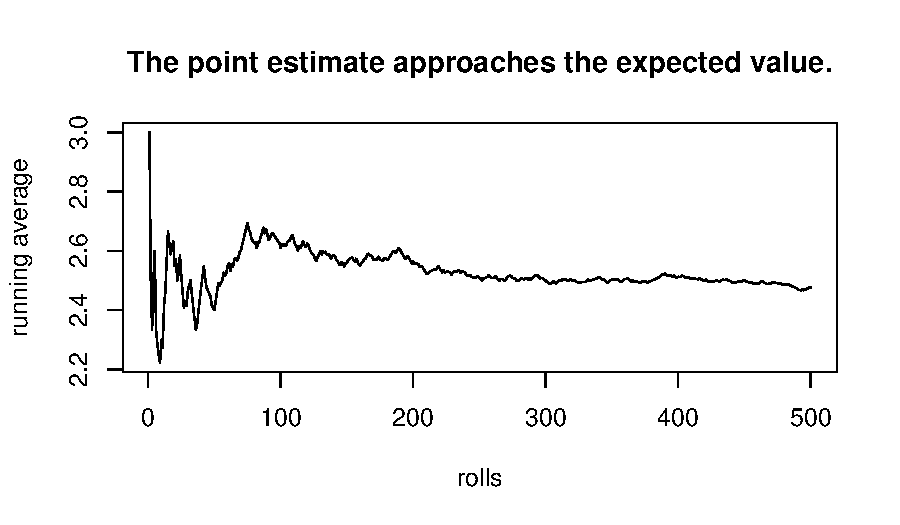
\includegraphics[width=0.7\textwidth]{4-1_var_in_est/figures/running_mean_4sided_die/running_die.pdf}
\end{center}
\vfill
\end{frame}


\begin{frame}
\vspace{-10pt}
\begin{center}
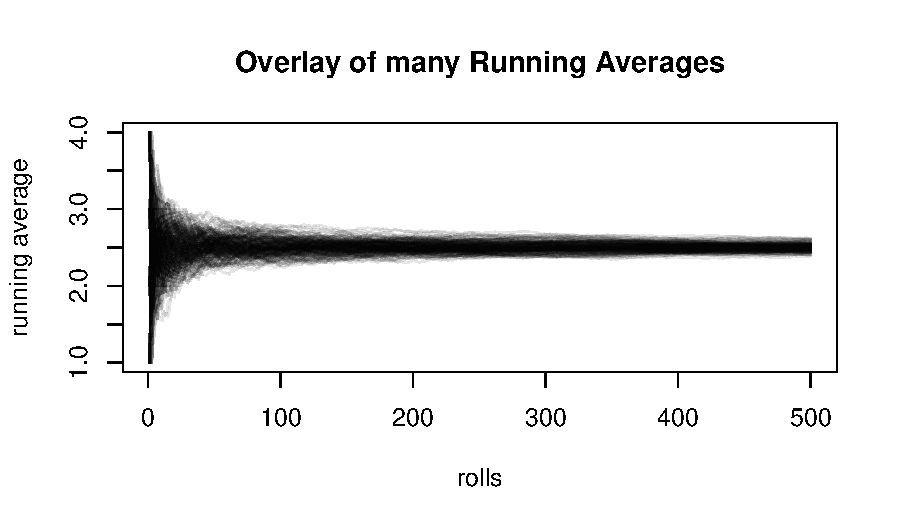
\includegraphics[width=\textwidth]{4-1_var_in_est/figures/running_mean_4sided_die/running_die_overlay.pdf}
\end{center}
\vspace{-20pt}
Notice the uncertainty gets smaller with larger sample size. However, there are diminishing returns...

The accuracy improves drastically from $n=1$ to $n=100$, but not nearly as drastically from $n=401$ to $n=500$.
\end{frame}



\begin{frame}[fragile]
Now, imagine we sample from a new population/distribution, but we don't know the population parameters. What can we conclude?
\begin{columns}
\begin{column}{0.6\textwidth}
\vspace{-20pt}
\begin{center}
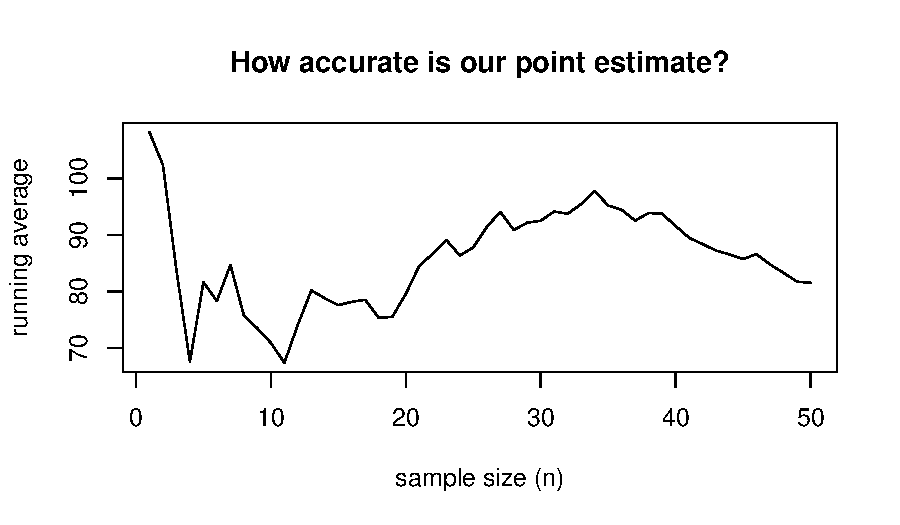
\includegraphics[width=\textwidth]{4-1_var_in_est/figures/running_mean_4sided_die/running_weight.pdf}
\end{center}
\vspace{-30pt}
\begin{center}
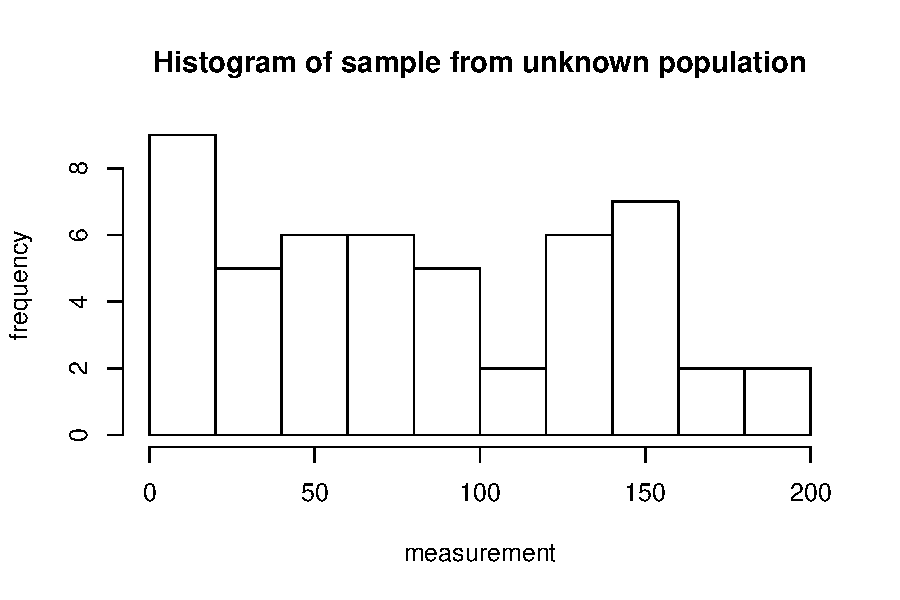
\includegraphics[width=\textwidth]{4-1_var_in_est/figures/running_mean_4sided_die/weight_hist.pdf}
\end{center}
\end{column}
\begin{column}{0.3\textwidth}
\pause
\soln{Well, our point estimate is $$\mu \approx \bar{x} = 26.4$$
However, we want to also describe our uncertainty. To me, based on the previous slide, I'd guess the uncertainty is about $\pm 1/10$ of the range?
$$\mu = 26.4 \pm 5 $$
}
\end{column}
\end{columns}
\end{frame}


\begin{frame}
\frametitle{Standard error}
Standard error quantifies our uncertainty of a point estimate.
$$SE = \frac{\sigma}{\sqrt{n}} $$
\pause
Remember the 4-sided die. That distribution has $\sigma = 1.118$. We can plot $\mu \pm SE$ as a function of $n$.
\begin{center}
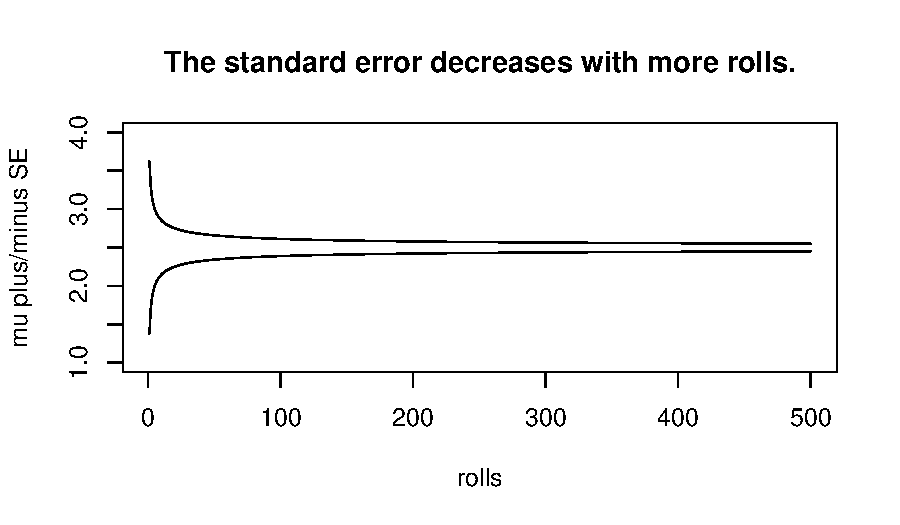
\includegraphics[width=0.8\textwidth]{4-1_var_in_est/figures/running_mean_4sided_die/running_die_SE.pdf}
\end{center}
\end{frame}


\begin{frame}
Let's return to our sample from an unknown population.
\begin{center}
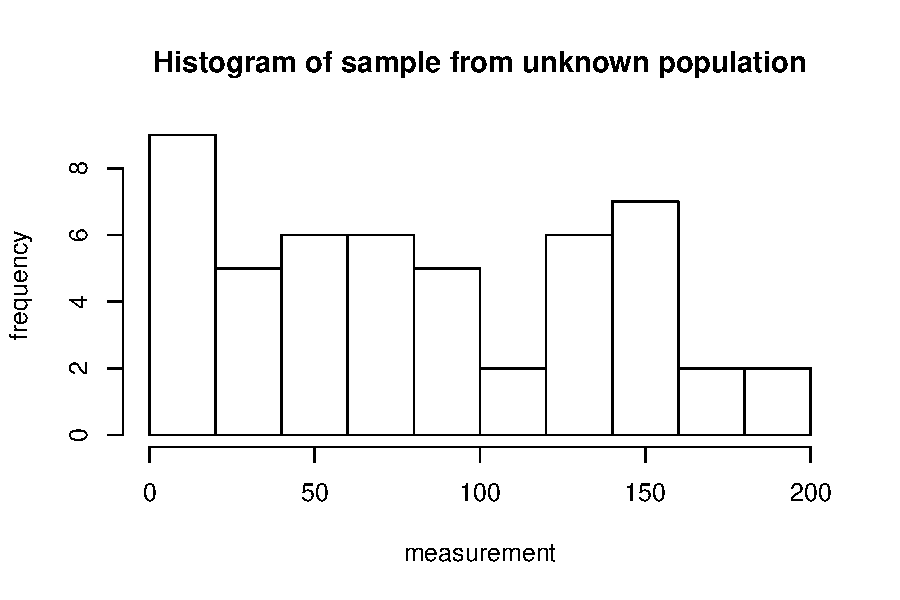
\includegraphics[width=0.7\textwidth]{4-1_var_in_est/figures/running_mean_4sided_die/weight_hist.pdf}
\end{center}
We do not know $\sigma$. \pause We can estimate $\sigma$ from $s$. \pause I calculated $s=15.5$.\pause
$$SE \approx \frac{15.5}{\sqrt{50}} = 2.19$$
\pause
So we think our estimate $\mu \approx \bar{x} = 26.4$ has an ``uncertainty'' of 2.19. But we need to define SE better...
\end{frame}


\begin{frame}
\frametitle{Sampling Distributions}
Let $X_i$ be the $i$th draw from a population. Let $n$ represent the number of draws. Let $Y$ be the average of those draws.
$$Y = \frac{\sum\limits_{i=1}^n X_i}{n}$$
By using the rules of Ch 2.4 we can show
$$\mu_Y = \mu_X$$
$$\sigma_{Y} = \cfrac{\sigma_X}{\sqrt{n}} $$
We say $Y$ is determined by a sampling distribution. That sampling distribution has the same mean as the population, but it has a smaller standard deviation (and its SD shrinks as $n$ increases). The SD of $Y$ is the SE.
 $$SE = \sigma_Y$$. 
\end{frame}


\begin{frame}
\frametitle{Sampling Distributions}
Let $X_i$ be the $i$th draw from a population. Let $n$ represent the number of draws. Let $\bar{X}$ be the average of those draws.
$$\bar{X} = \frac{\sum\limits_{i=1}^n X_i}{n}$$
By using the rules of Ch 2.4 we can show
$$E(\bar{X}) = E(X)$$
$$SD(\bar{X}) = \cfrac{SD(X)}{\sqrt{n}} $$

The book also uses $SD_{\bar{x}}$ to represent standard error.
$$SE =SD(\bar{X}) = SD_{\bar{x}} $$

\end{frame}








\begin{frame}
\frametitle{Sampling Simulations}
Let's roll 6-sided dice (on a computer to save time). 
\vspace{-20pt}
\begin{columns}
\begin{column}{0.5\textwidth}
\begin{center}
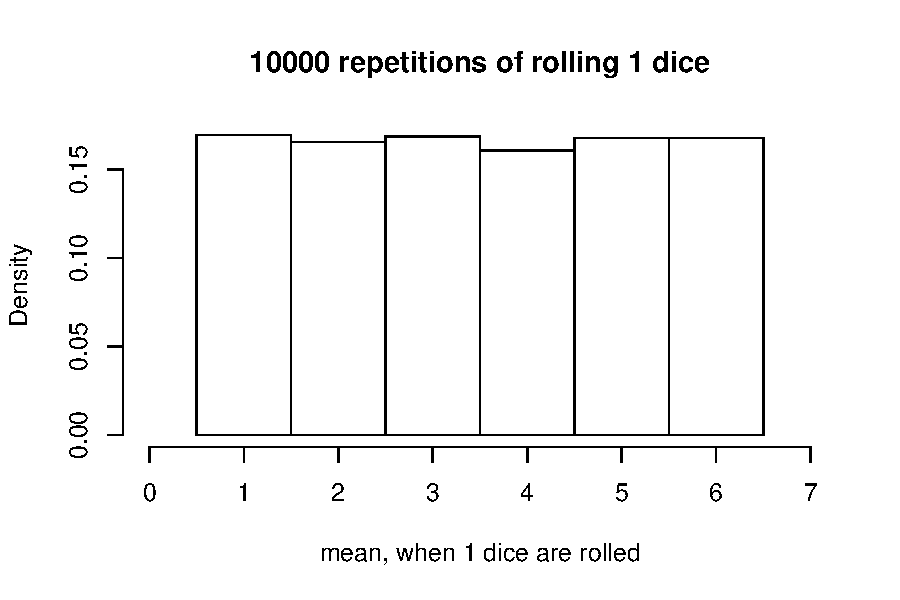
\includegraphics[width=0.9\textwidth]{4-1_var_in_est/figures/six_sided_dice/rolls_by_1.pdf}

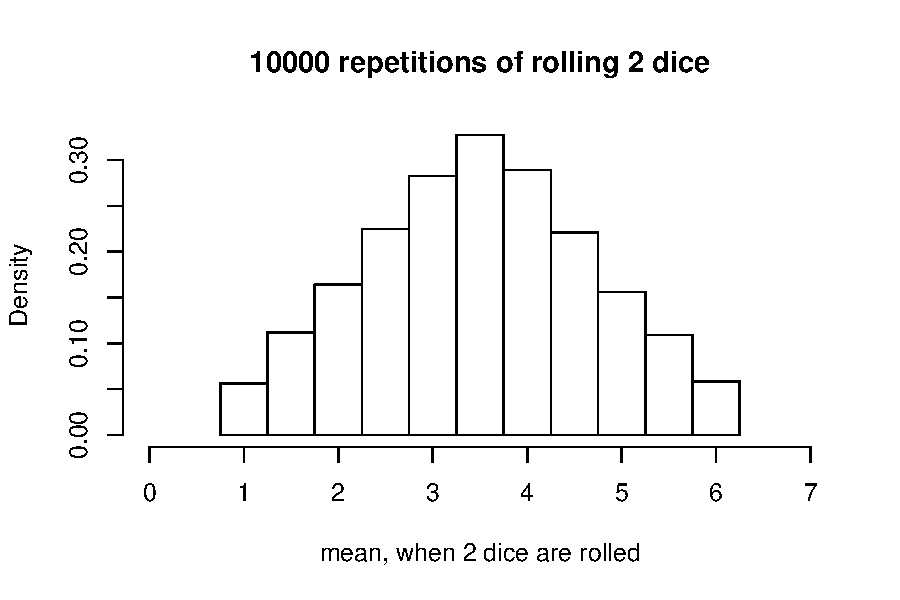
\includegraphics[width=0.9\textwidth]{4-1_var_in_est/figures/six_sided_dice/rolls_by_2.pdf}
\end{center}
\end{column}
\begin{column}{0.5\textwidth}
\begin{center}
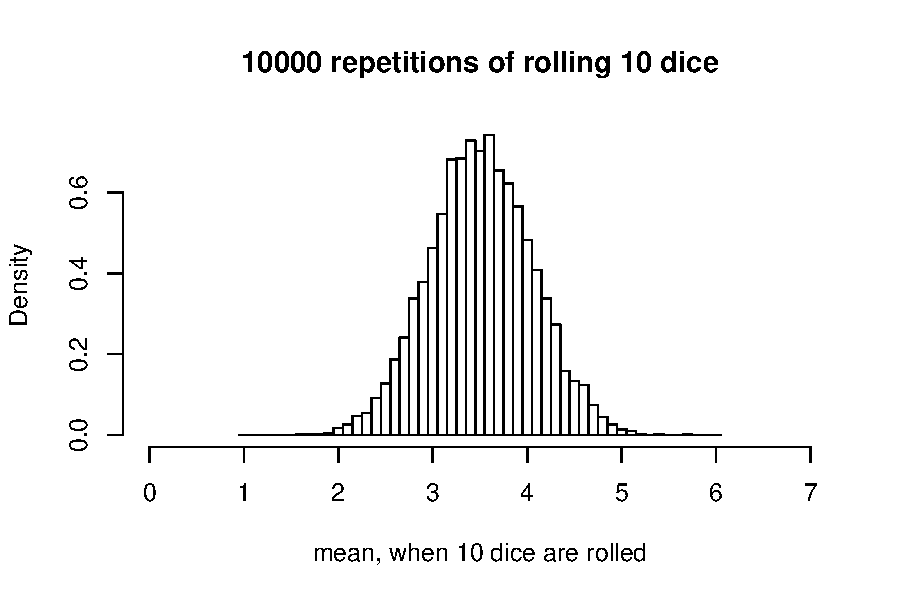
\includegraphics[width=0.9\textwidth]{4-1_var_in_est/figures/six_sided_dice/rolls_by_10.pdf}

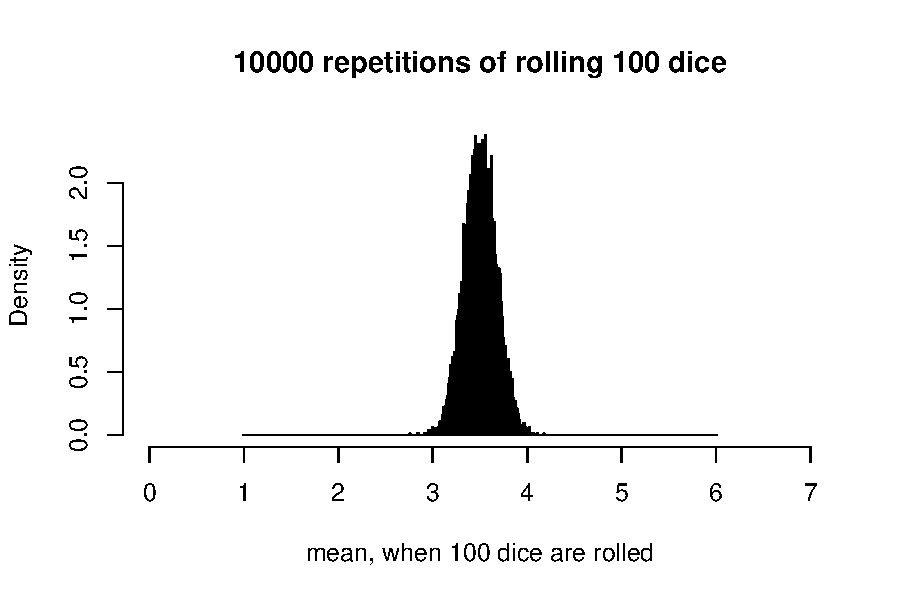
\includegraphics[width=0.9\textwidth]{4-1_var_in_est/figures/six_sided_dice/rolls_by_100.pdf}
\end{center}
\end{column}
\end{columns}
\end{frame}



\begin{frame}
\frametitle{Practice}
\vspace{-20pt}
\begin{center}
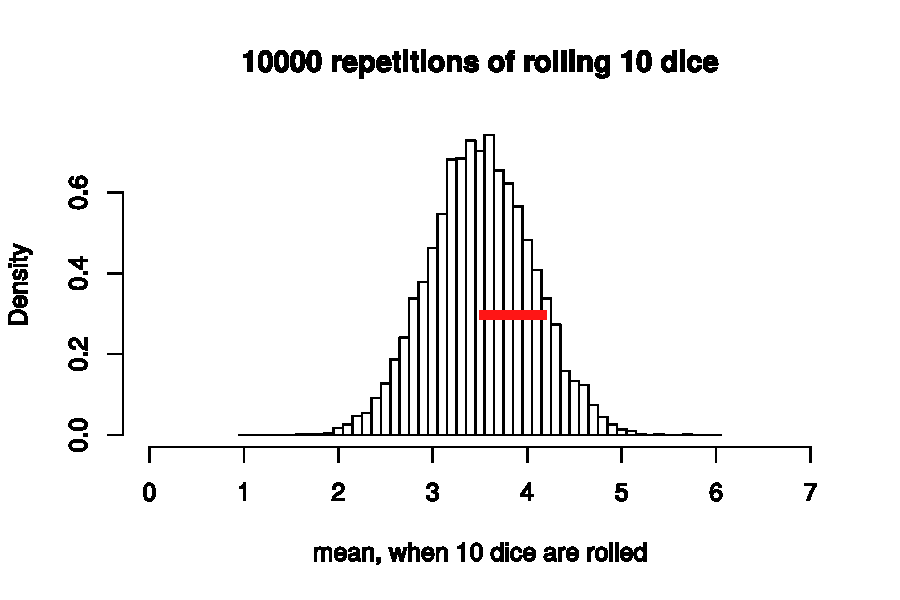
\includegraphics[width=0.6\textwidth]{4-1_var_in_est/figures/six_sided_dice/rolls_by_10_SE.pdf}
\end{center}
\vspace{-20pt}Estimate the standard error when rolling 10 dice at a time.

\pause \soln{Notice the sampling distribution looks nearly normal. I estimate that the standard deviation looks to be about {\bf 0.7}?}
\vfill
\pause
I calculated that for rolling a single die, $\sigma = 2.92$. Calculate the standard error when rolling 10 dice.
\soln{$$SE = \frac{2.92}{\sqrt{10}} = 0.922$$}
\vfill
\end{frame}
